% !Mode:: "TeX:UTF-8"
\section{问题描述}

本研究旨在分析不同算数能力人群在进行算数任务前后的EEG信号差异。从36个受试者中随机选取2个算数能力好的(Group G)和2个算数能力差的(Group B)，对两组人在进行算数任务前后的EEG信号进行AR(p)建模分析，比较AR模型阶数、AR谱以及其他EEG特征的差异。

数据来源于EEG脑电数据集，包含36名受试者的脑电记录：
- Group G（算数能力好）：24名受试者，平均每4分钟完成21次运算
- Group B（算数能力差）：12名受试者，平均每4分钟完成7次运算

每个受试者包含两个EDF格式文件：
- \_1文件：算数任务前的背景EEG记录
- \_2文件：算数任务期间的EEG记录

\section{AR模型原理}

自回归模型（AutoRegressive Model, AR）是一种常用的时间序列分析方法。AR(p)模型假设当前时刻的信号值可以由其前p个时刻的值线性组合而成：

\[
x(n) = \sum_{k=1}^{p} a_k x(n-k) + u(n)
\]

其中：
- \( x(n) \) 是n时刻的信号值
- \( p \) 是模型阶数
- \( a_k \) 是AR系数
- \( u(n) \) 是白噪声输入

AR模型的阶数选择采用Akaike信息准则（AIC）：
\[
AIC = n \cdot \ln(\sigma^2) + 2p
\]

其中\( \sigma^2 \)是残差方差，选择使AIC最小的阶数。

AR谱通过对AR系数进行Z变换得到功率谱估计：
\[
P_{AR}(f) = \frac{\sigma^2}{\left|1 - \sum_{k=1}^{p} a_k e^{-j2\pi f k / f_s}\right|^2}
\]

\section{实验方法}

\subsection{数据选择}
从Group G中随机选取Subject22和Subject04，从Group B中随机选取Subject24和Subject28。

\subsection{特征提取}
对每个受试者的所有EEG通道提取以下特征：
1. AR模型阶数（使用AIC准则估计）
2. AR谱估计
3. 传统功率谱密度（PSD，使用Welch方法）
4. Theta频段（4-8 Hz）功率
5. Alpha频段（8-13 Hz）功率
6. Beta频段（13-30 Hz）功率

\section{实验结果}

\subsection{AR模型阶数分析}

AR模型阶数分布如图~\ref{fig:ar_order}所示：

\begin{figure}[H]
    \centering
    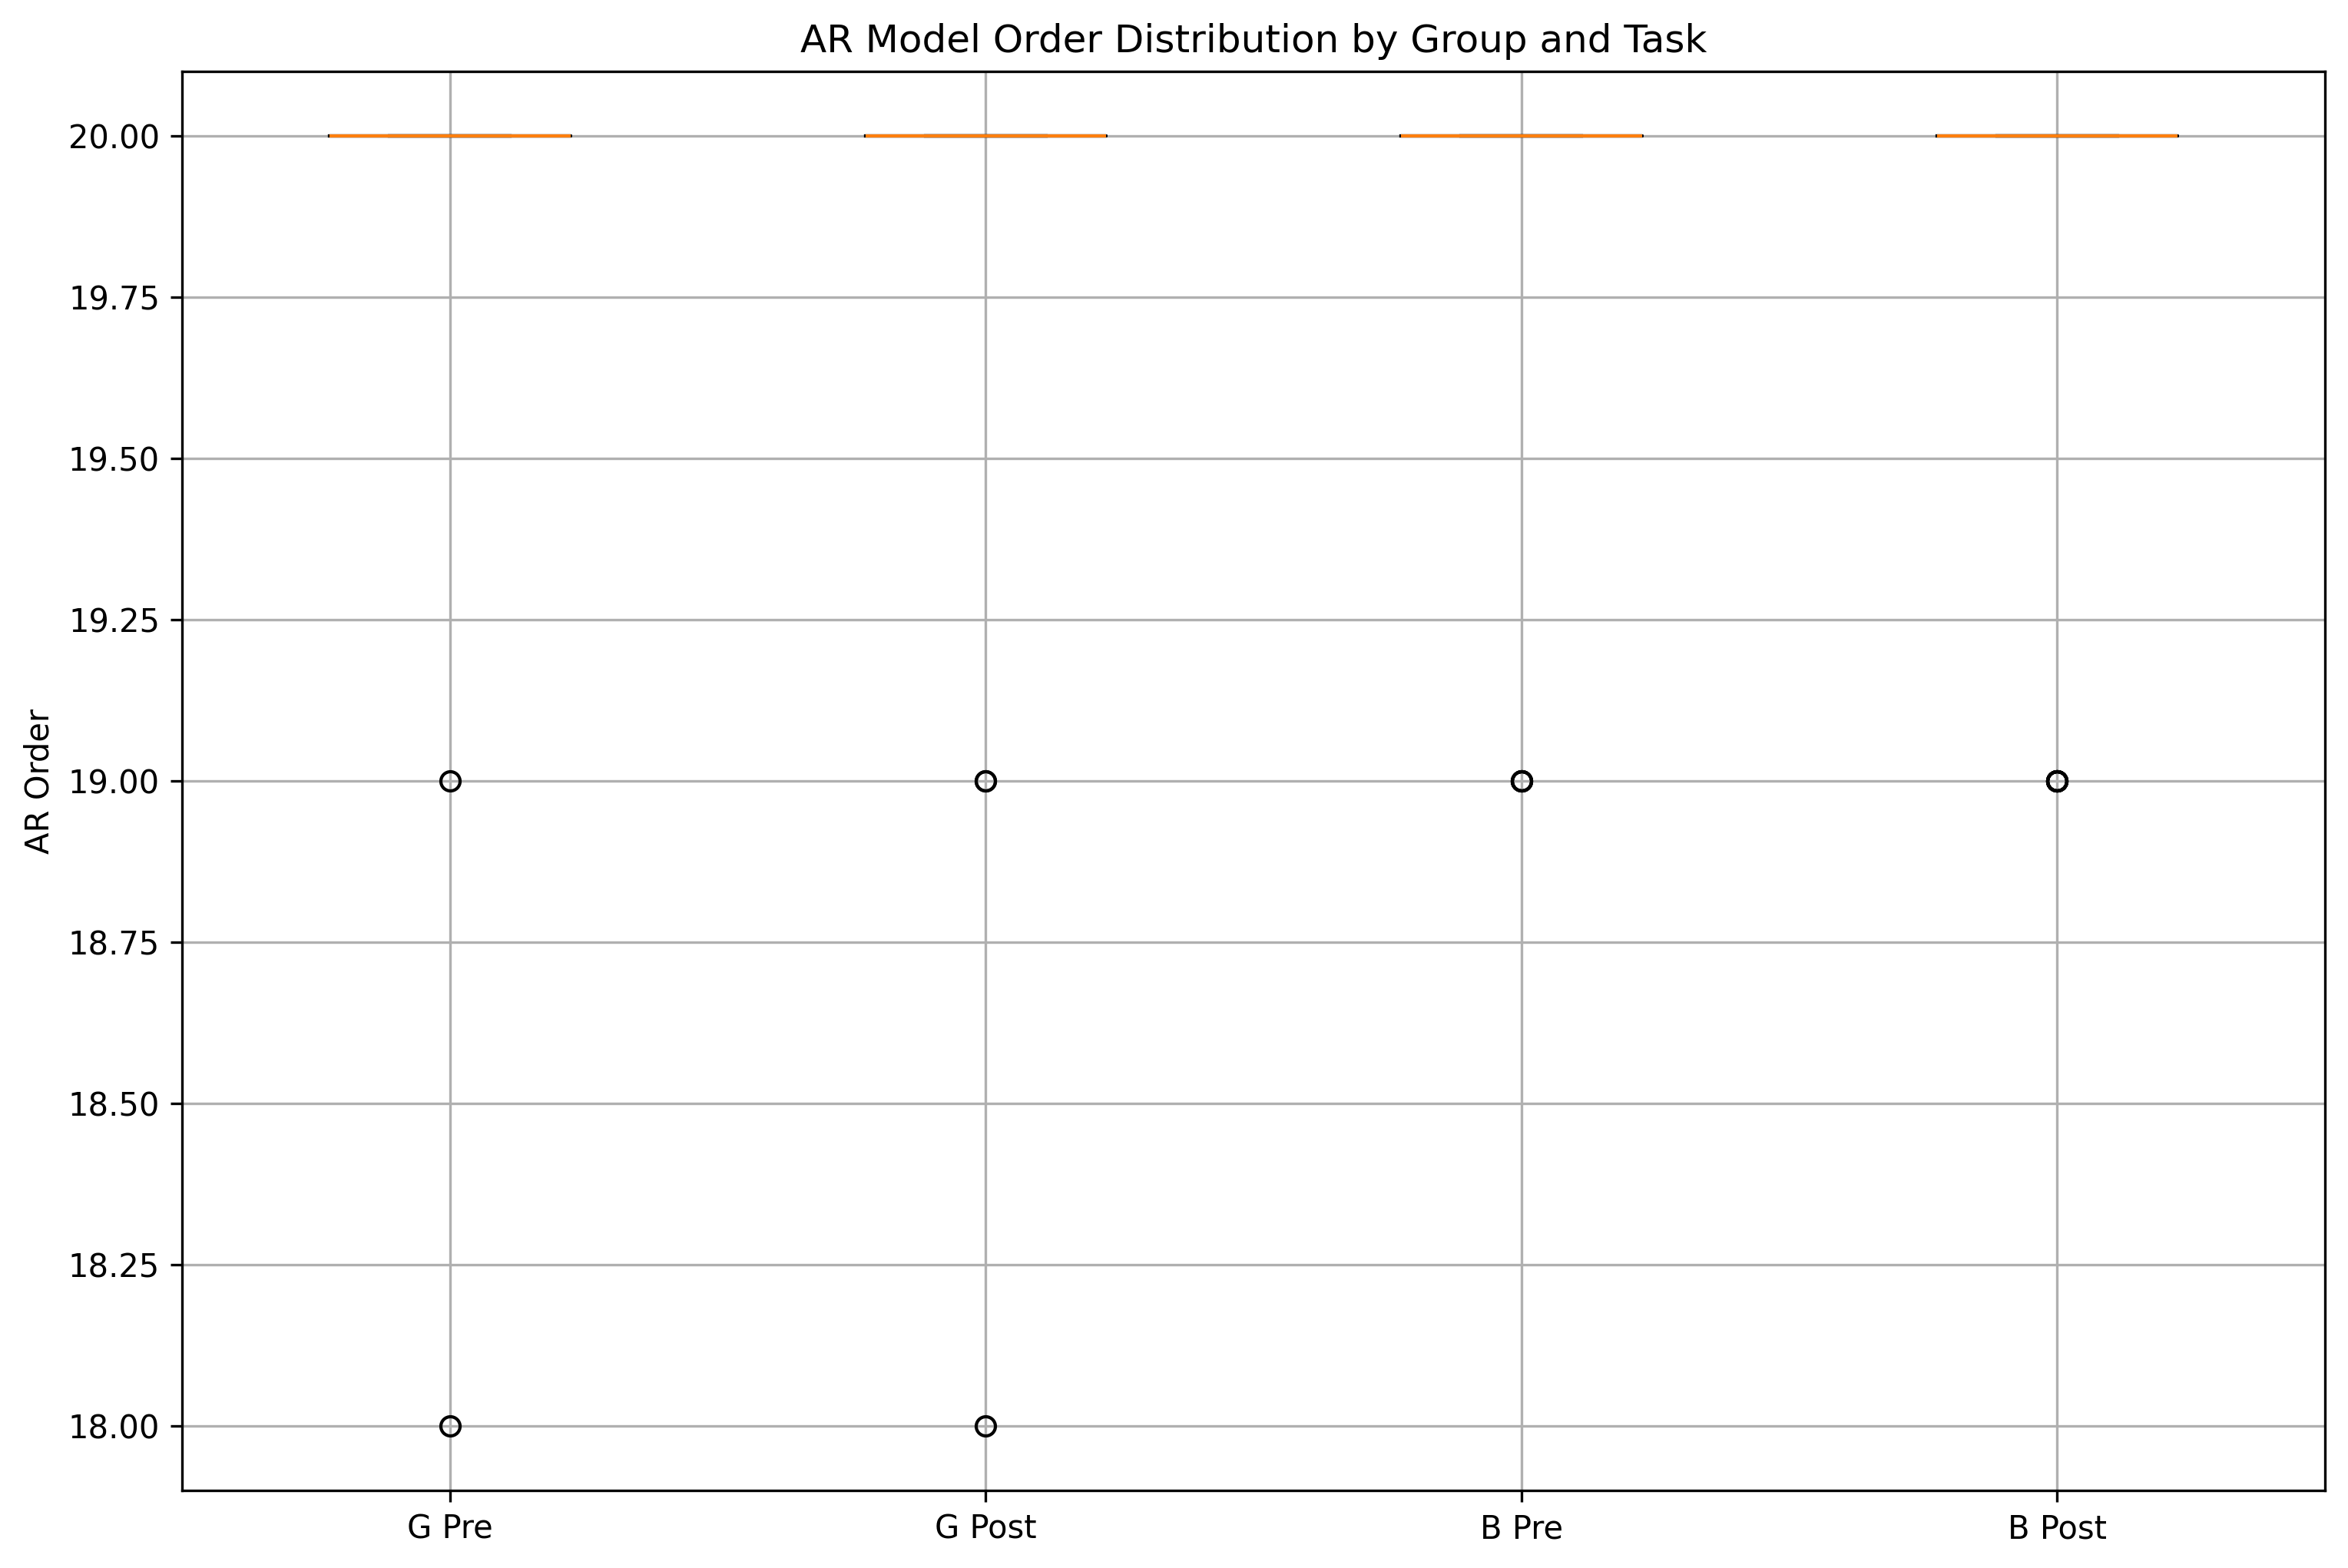
\includegraphics[width=0.8\textwidth]{figure/HW3figure/ar_order_boxplot.png}
    \caption{AR模型阶数分布箱线图}
    \label{fig:ar_order}
\end{figure}

从图中可以看出，所有组的AR模型阶数都接近最大值20，表明EEG信号具有复杂的时间结构，需要较高阶的模型才能准确描述。Group G和Group B之间的AR阶数差异较小。

\subsection{功率谱密度对比}

各组的平均功率谱密度如图~\ref{fig:psd}所示：

\begin{figure}[H]
    \centering
    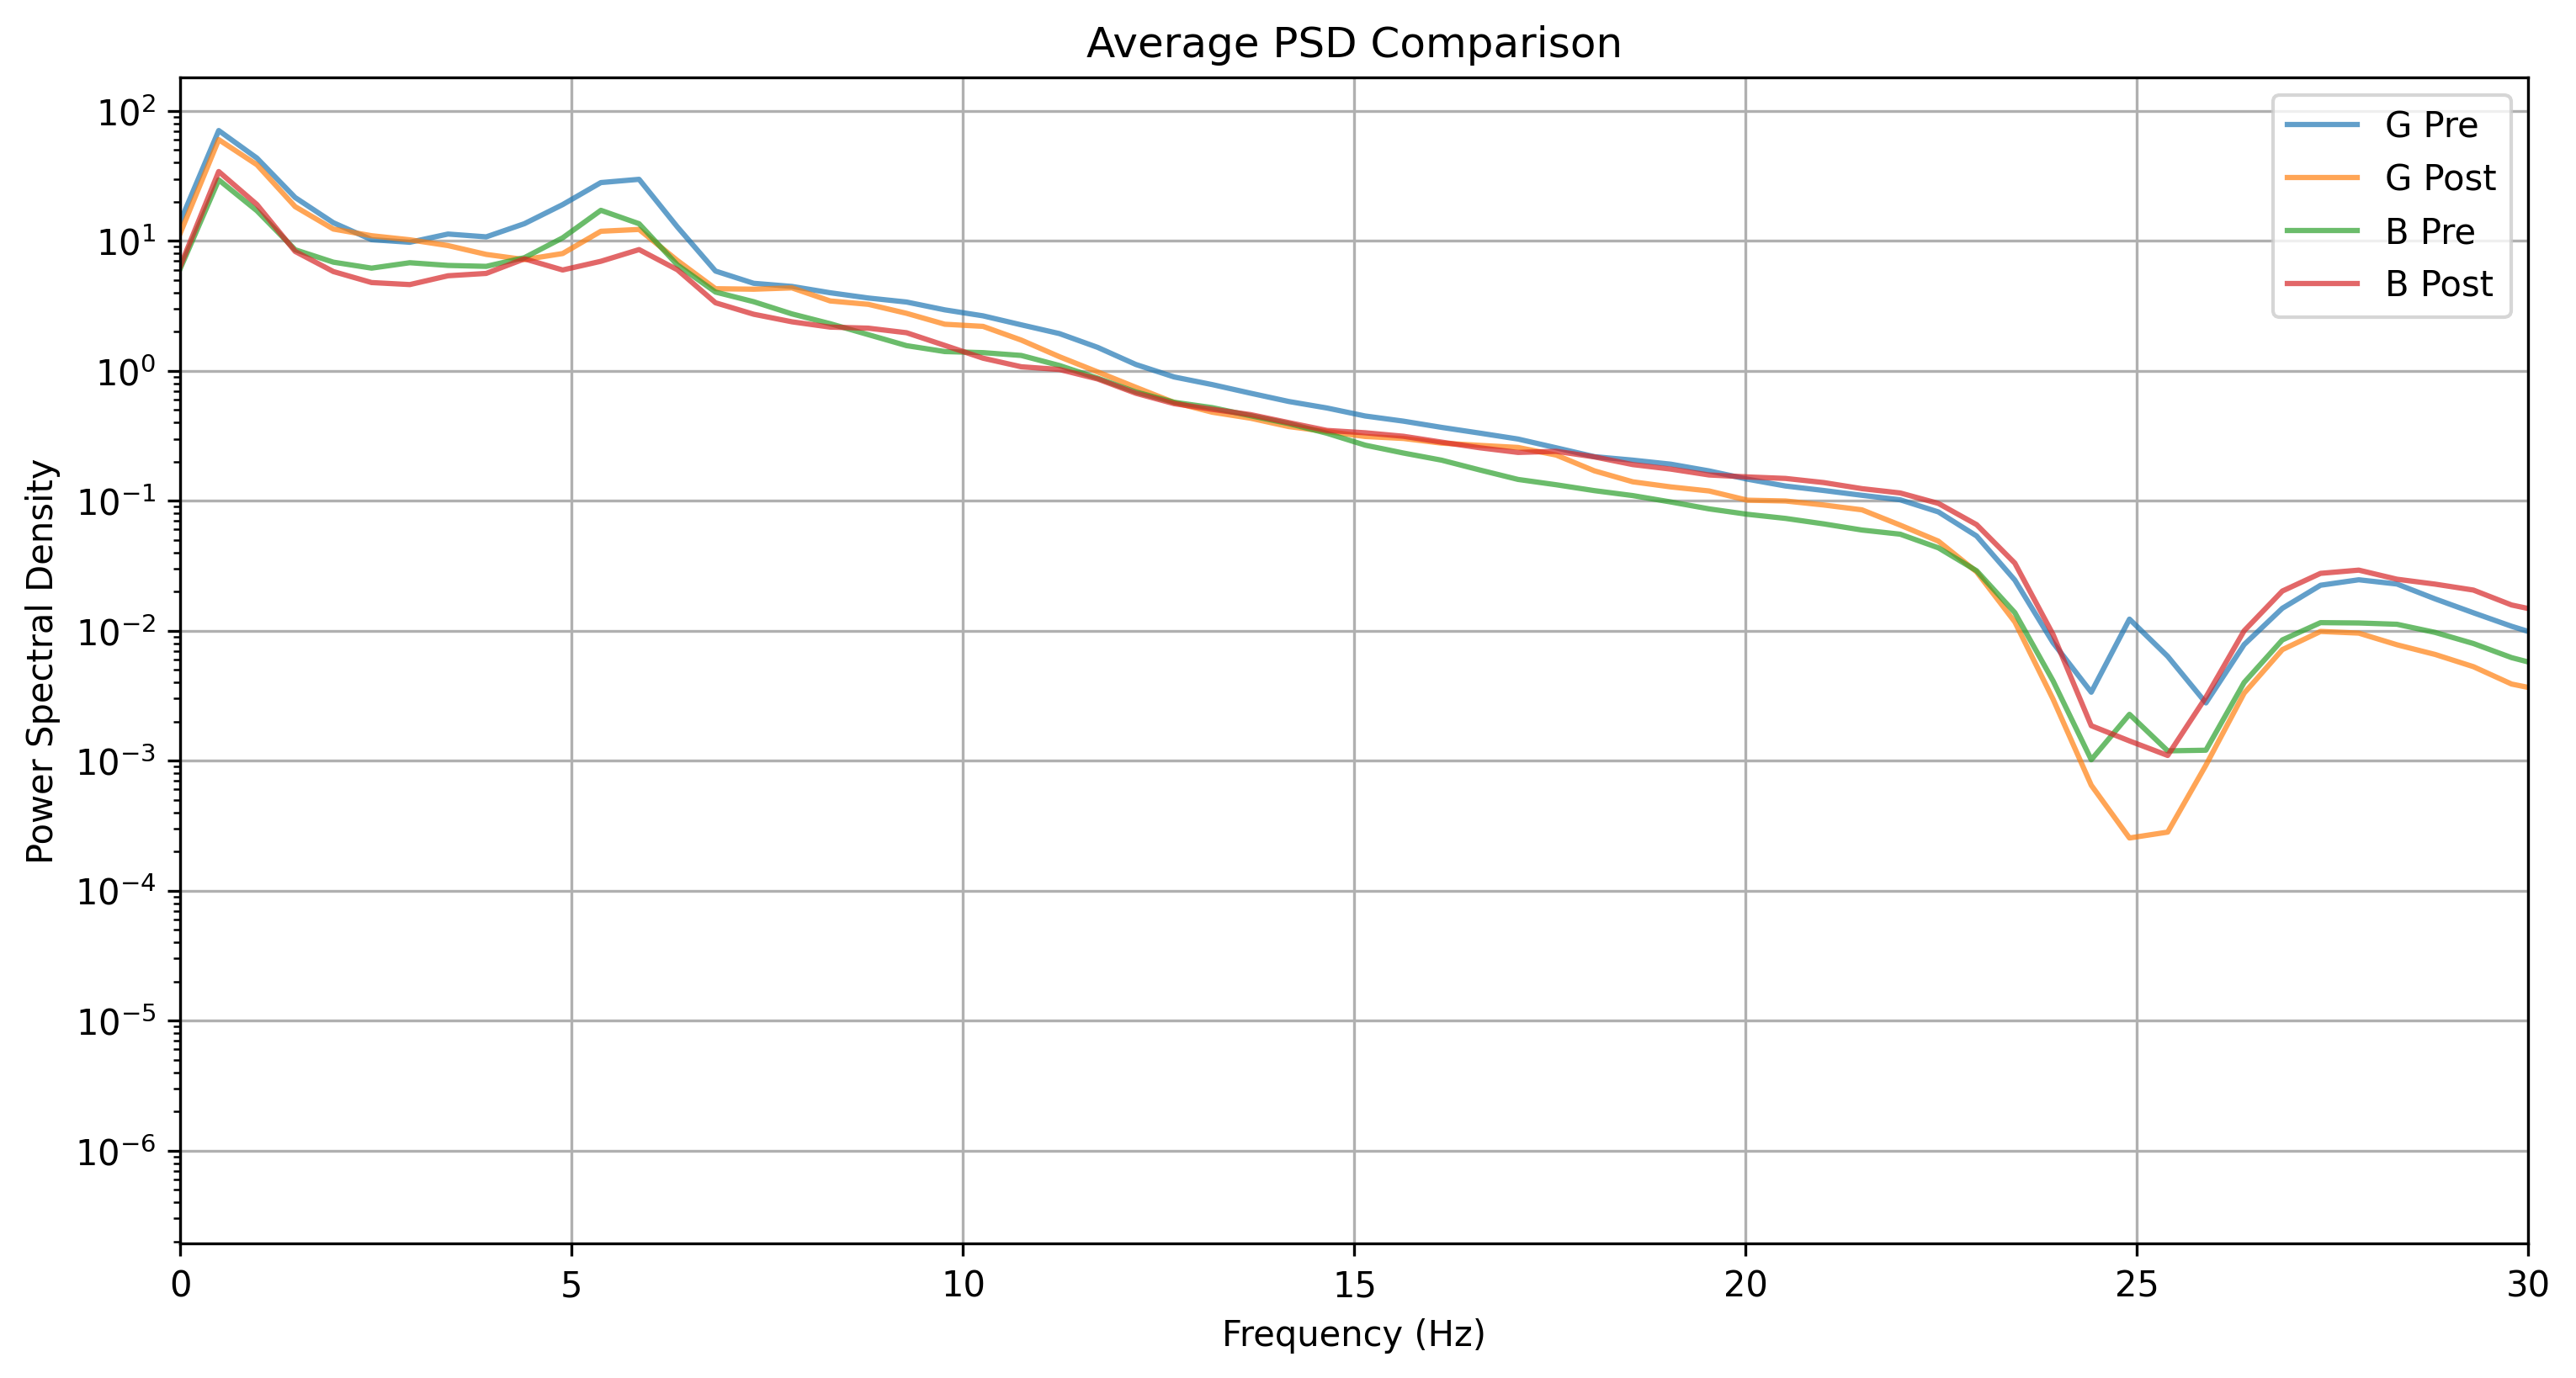
\includegraphics[width=0.8\textwidth]{figure/HW3figure/psd_comparison.png}
    \caption{平均功率谱密度对比}
    \label{fig:psd}
\end{figure}

可以观察到，算数任务后两组的整体功率都有所下降，尤其是在低频段。Group G在任务前的功率明显高于Group B。

\subsection{AR谱对比}

AR谱估计结果如图~\ref{fig:ar_spec}所示：

\begin{figure}[H]
    \centering
    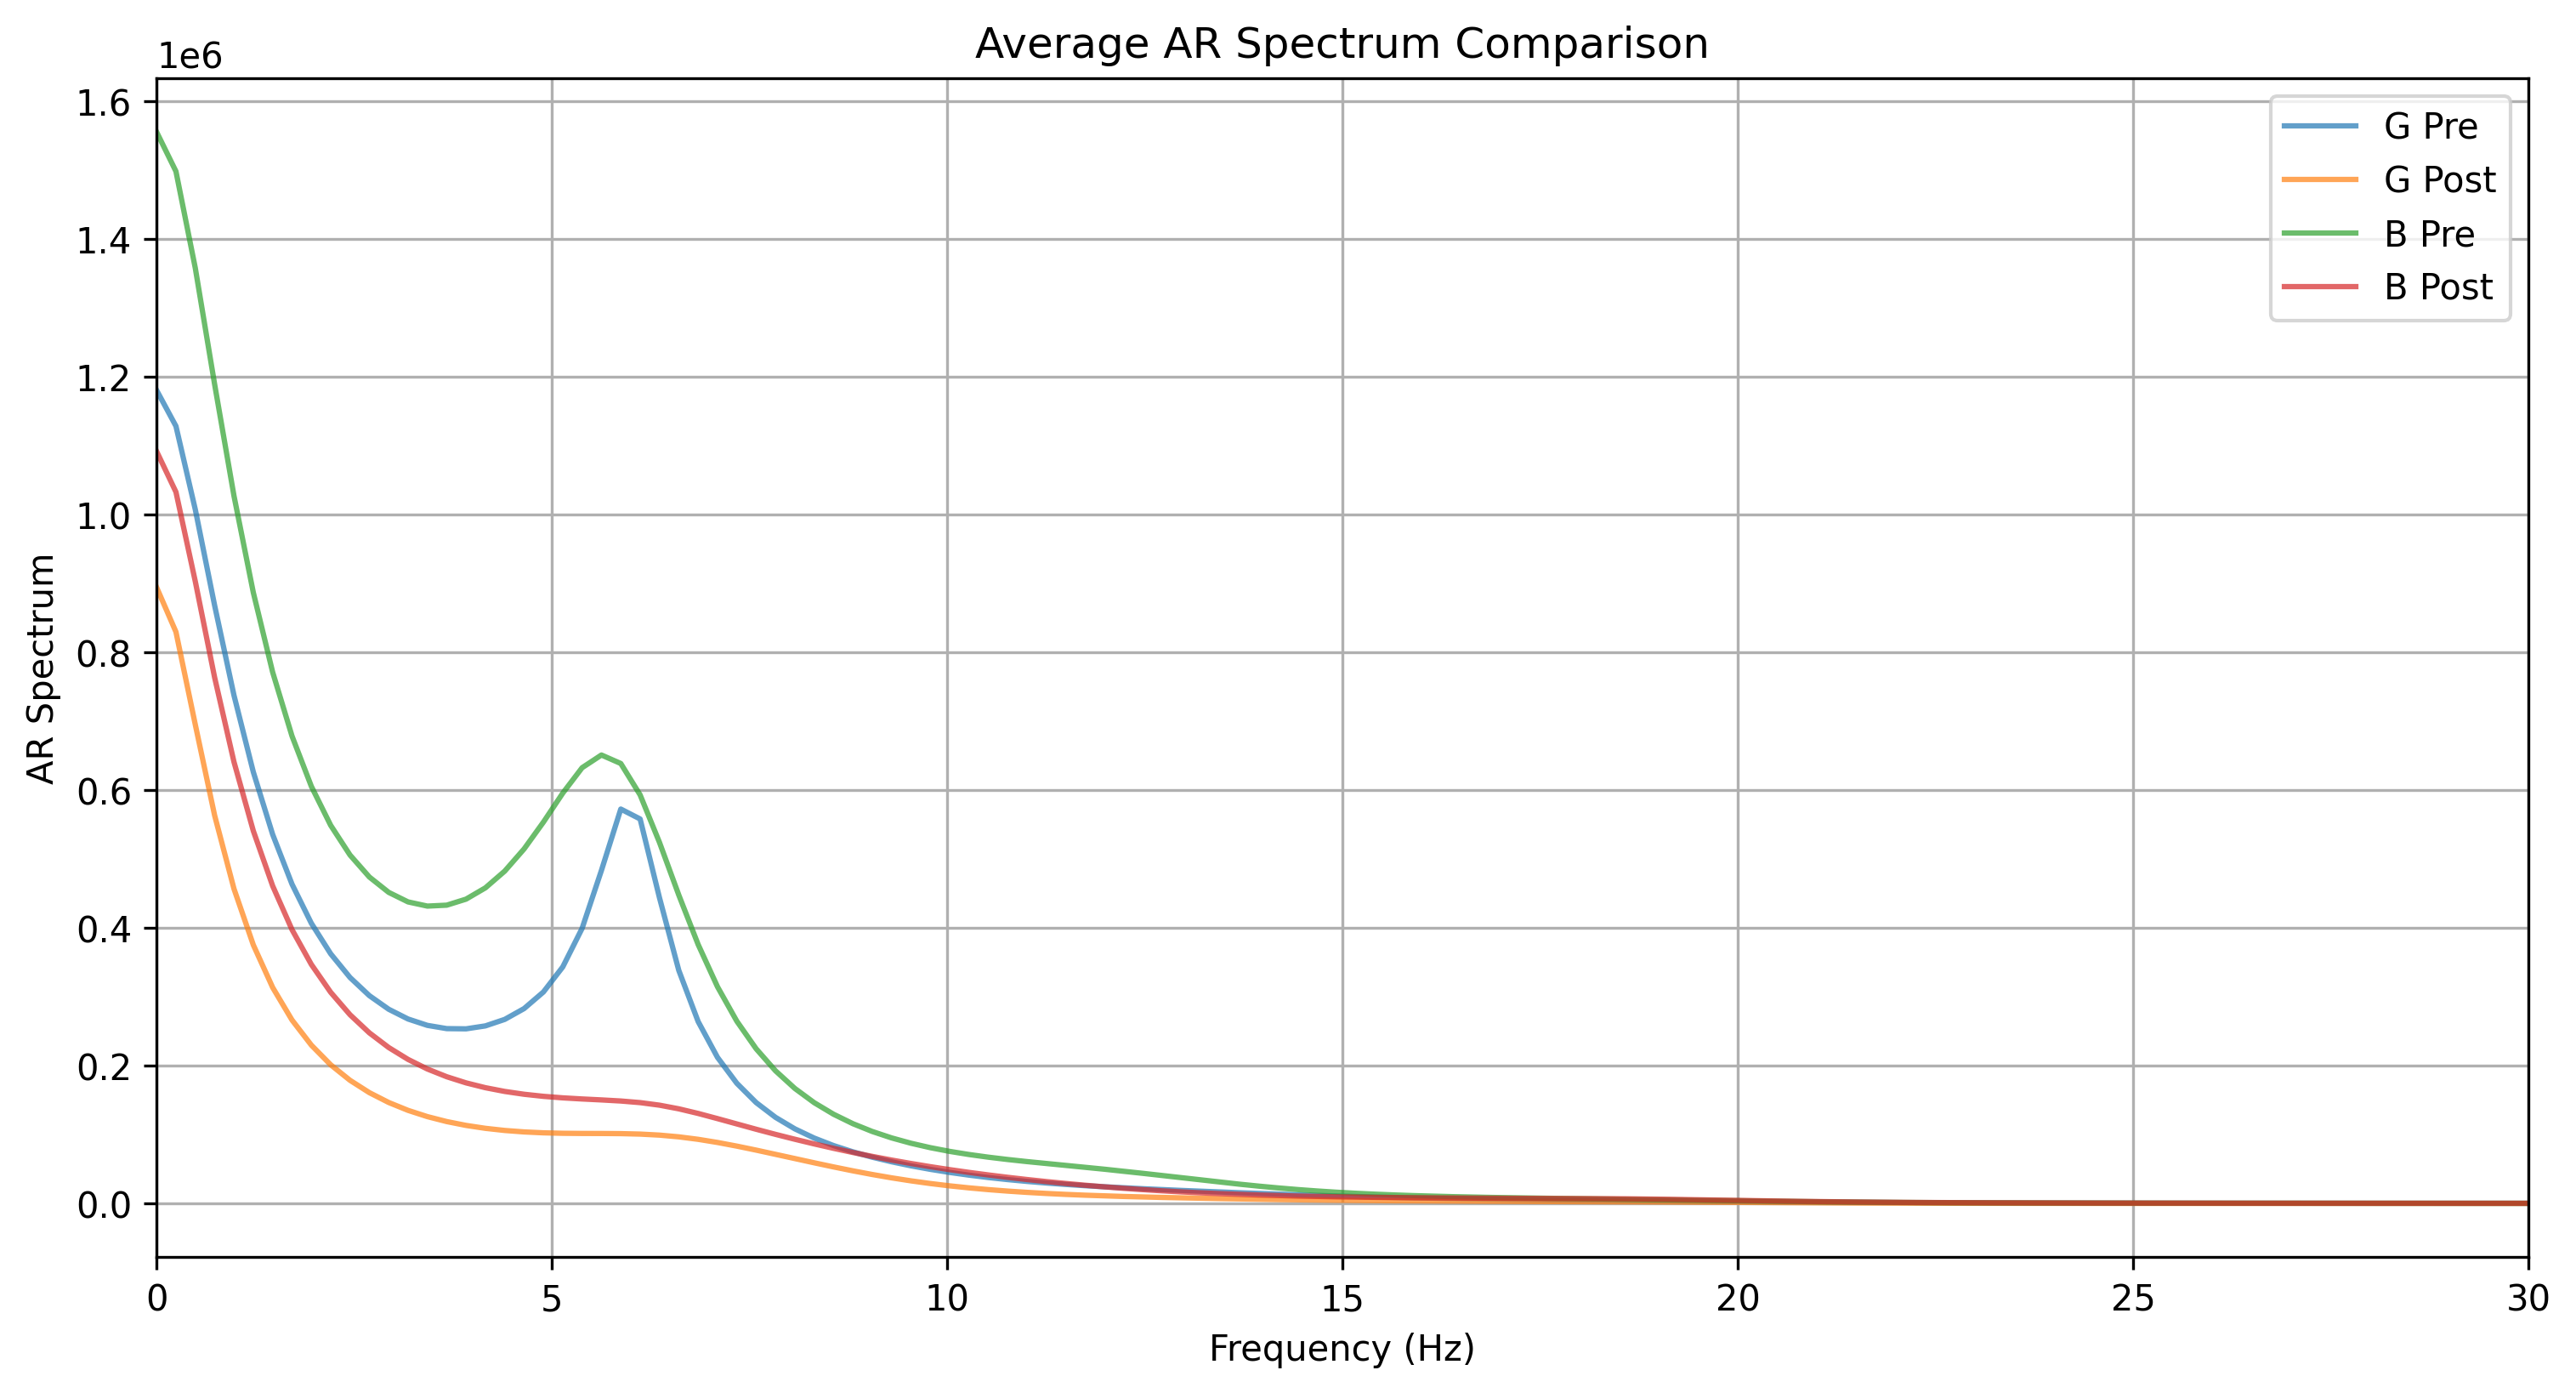
\includegraphics[width=0.8\textwidth]{figure/HW3figure/ar_spectrum_comparison.png}
    \caption{平均AR谱对比}
    \label{fig:ar_spec}
\end{figure}

AR谱与传统PSD呈现相似的趋势，但AR谱更加平滑，能够更好地捕捉信号的周期性成分。

\subsection{频段功率分析}

各频段功率统计如图~\ref{fig:band_power}所示：

\begin{figure}[H]
    \centering
    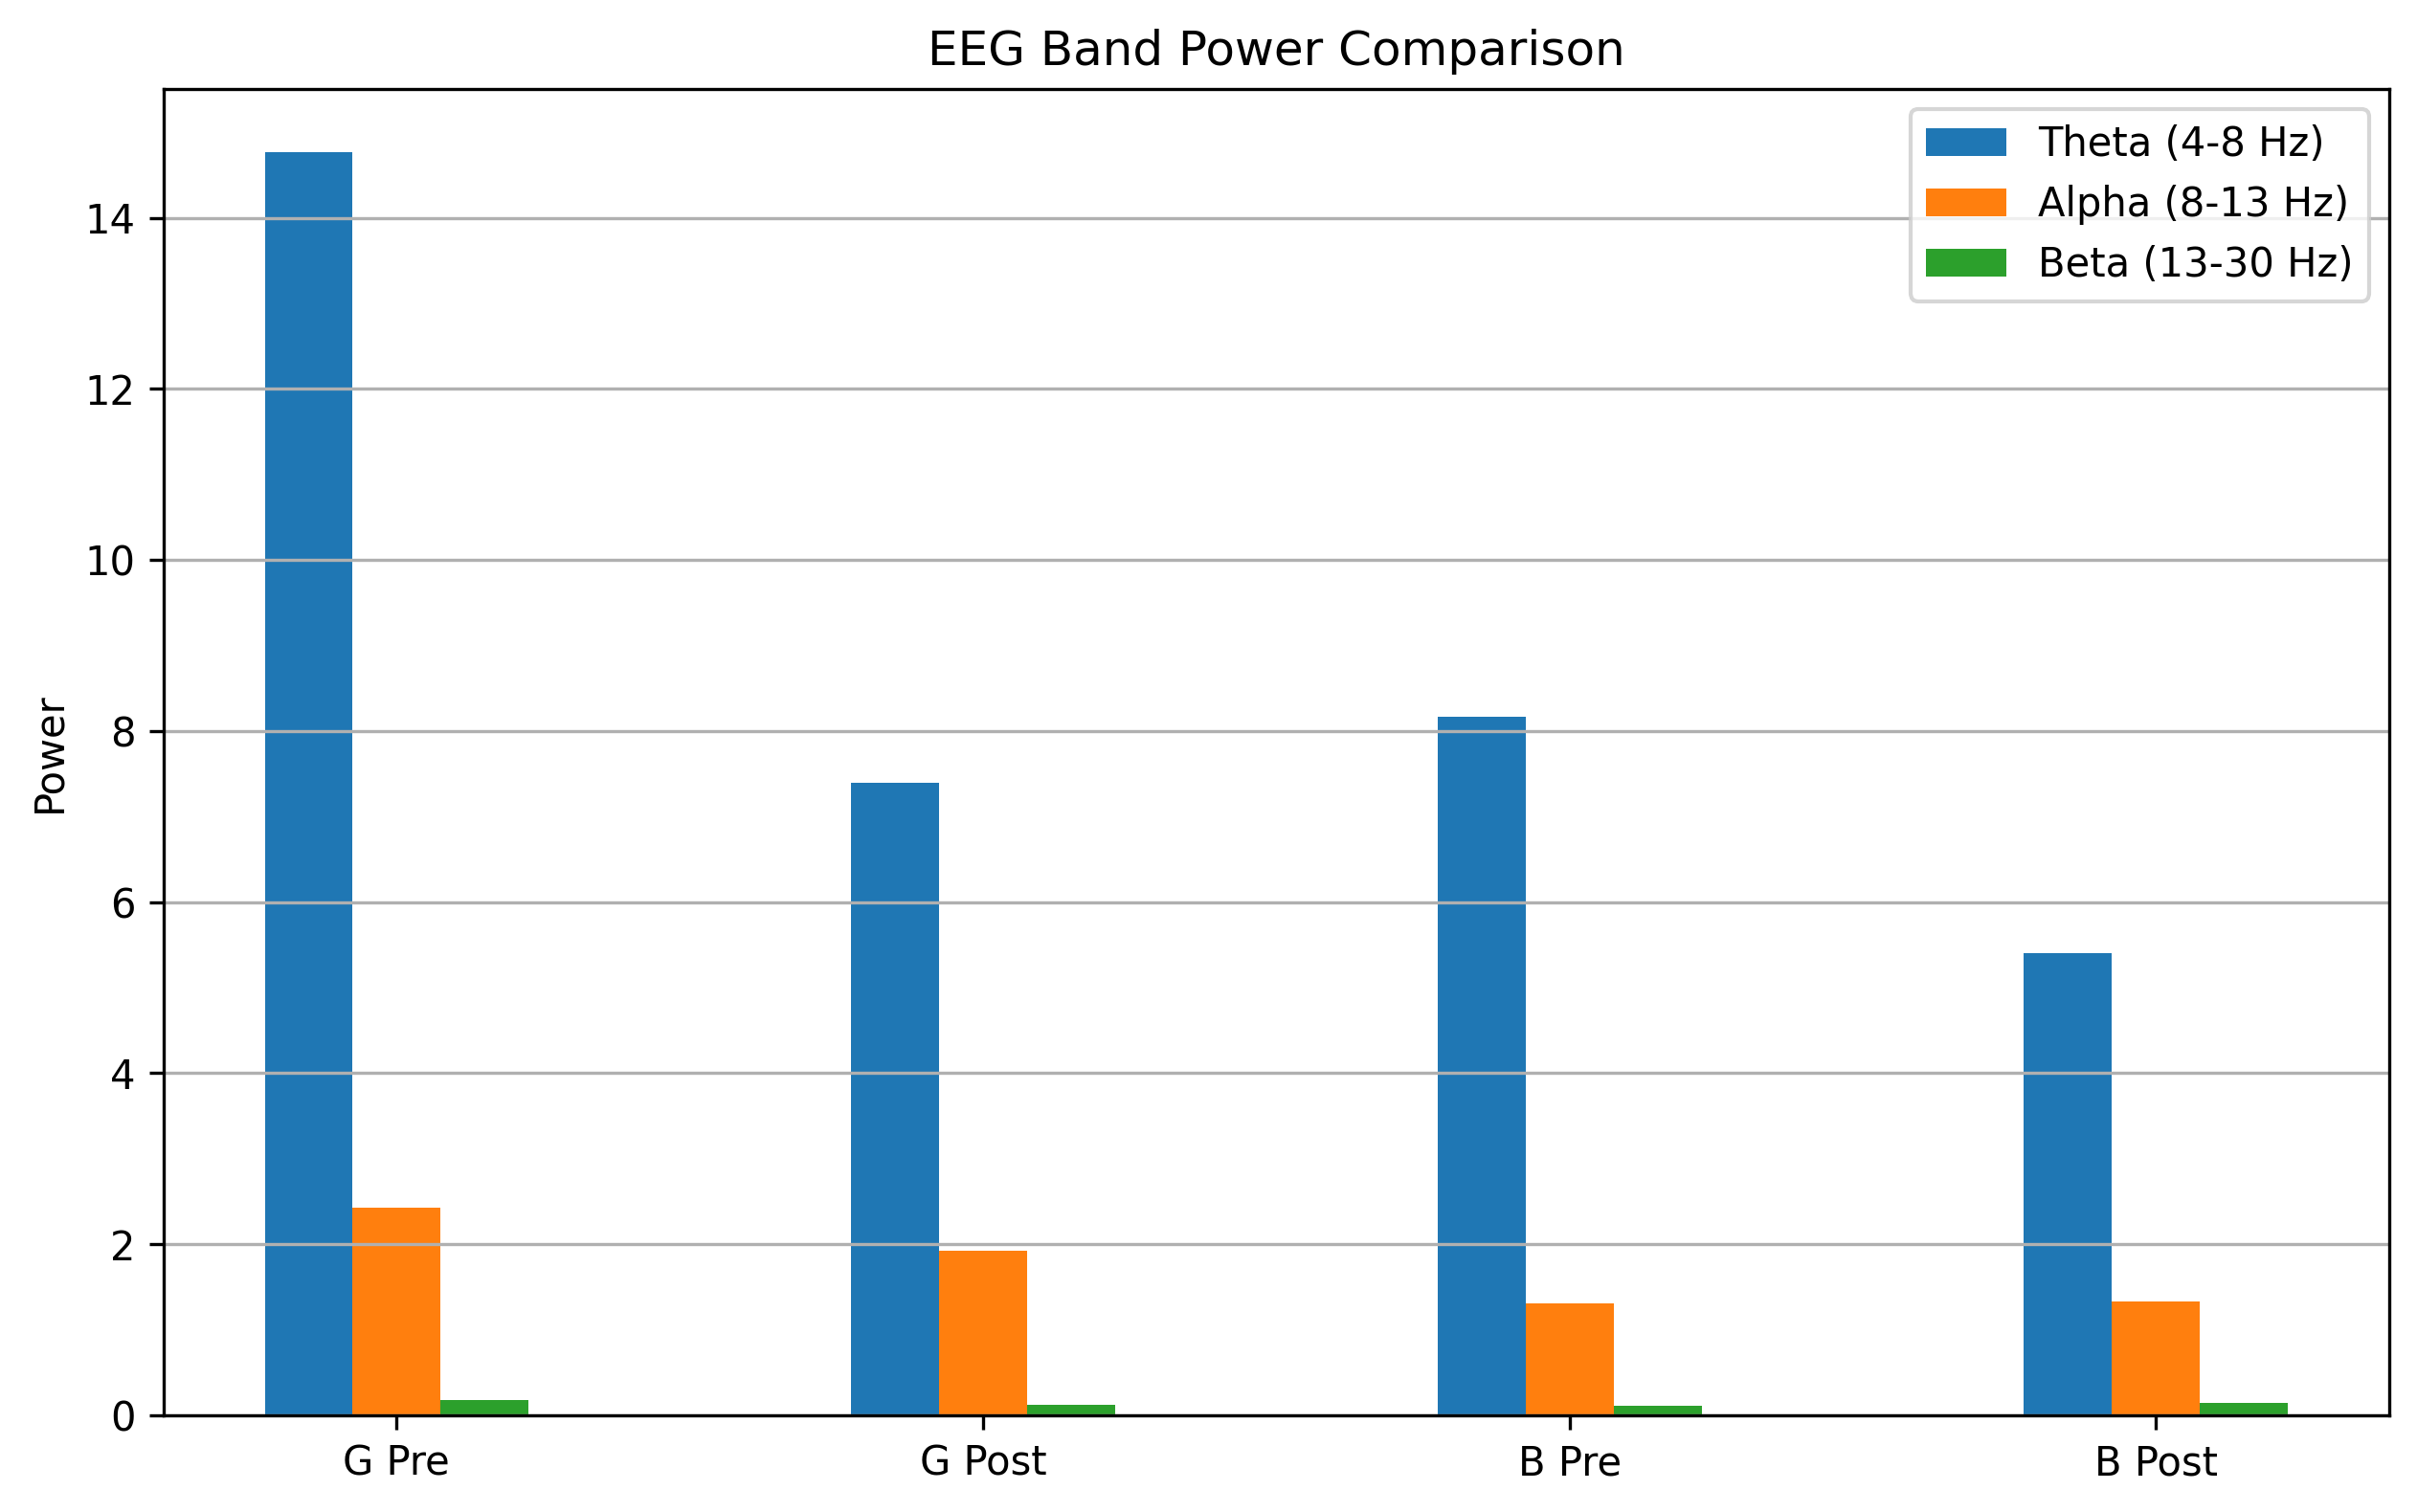
\includegraphics[width=0.8\textwidth]{figure/HW3figure/band_power_bar.png}
    \caption{各频段功率对比}
    \label{fig:band_power}
\end{figure}

\section{结果讨论}

\subsection{AR模型阶数差异}
从表~\ref{tab:stats}可以看出，所有组的AR模型阶数均值都接近20，说明EEG信号具有较高的时间复杂度。Group G和Group B之间的AR阶数差异不明显。

\begin{table}[H]
    \centering
    \caption{各组统计结果}
    \label{tab:stats}
    \begin{tabular}{|c|c|c|c|c|c|c|}
        \hline
        Group & Task & AR阶数均值 & Theta功率 & Alpha功率 & Beta功率 \\
        \hline
        G & Pre & 19.93 & 14.77 & 2.43 & 0.18 \\
        G & Post & 19.90 & 7.40 & 1.92 & 0.13 \\
        B & Pre & 19.90 & 8.17 & 1.31 & 0.11 \\
        B & Post & 19.83 & 5.40 & 1.33 & 0.15 \\
        \hline
    \end{tabular}
\end{table}

\subsection{Theta频段差异}
Group G在任务前的Theta功率显著高于Group B（14.77 vs 8.17），这可能反映了算数能力好的受试者在休息状态下大脑具有更高的认知准备状态。任务后，两组的Theta功率都下降，但Group G的下降幅度更大（约50\% vs 34\%）。

\subsection{Alpha频段差异}
Group G的Alpha功率在任务前后均高于Group B，且任务后明显下降。Alpha波通常与放松状态相关，任务期间Alpha波减少表明大脑处于活跃状态。

\subsection{Beta频段差异}
Beta功率在两组间差异较小，但Group B在任务后Beta功率略有上升，而Group G则下降。Beta波与注意力和认知加工相关，这可能表明两组在认知策略上存在差异。

\section{结论}

通过对随机选取的4名受试者进行AR模型分析，得到以下结论：

\begin{itemize}
    \item AR模型阶数在所有组中均接近20，表明EEG信号需要高阶模型描述，两组间阶数差异不显著；
    \item Group G在任务前的Theta和Alpha功率显著高于Group B，可能反映了更好的认知准备状态；
    \item 算数任务后，Group G的Theta和Alpha功率下降幅度更大，表明其大脑活动变化更明显；
    \item AR谱与传统PSD分析结果一致，但AR谱更平滑，适合分析EEG信号的周期性成分。
\end{itemize}

本研究表明，AR模型可以有效用于EEG信号分析，不同算数能力人群在EEG特征上存在显著差异。

\section{代码附录}
\lstinputlisting[language=Python]{codes/HW3codes/eeg_ar_analysis.py}